\documentclass[a4paper,12pt]{article}

\usepackage{rotating}
\usepackage[top=0.75in, bottom=0.75in, left=0.75in, right=0.75in]{geometry}
\usepackage{graphicx}
\usepackage[numbers,square,sort&compress]{natbib}
\usepackage{setspace}
\usepackage[cdot,mediumqspace,]{SIunits}
\usepackage{caption}
\usepackage{subcaption}
\usepackage{mathtools}
\usepackage{authblk}
\usepackage{wrapfig}
\usepackage[title,titletoc,toc]{appendix}
\providecommand{\e}[1]{\ensuremath{\times 10^{#1}}}

\begin{document}
\onehalfspacing
\title{Orbit Determination From Astrometry of Asteroids Ceres and Urania}
\author{Natalie Price-Jones, with lab partners Patrick Dorval and Jessica Campbell}
\date{3 February, 2014}
\affil{\small{natalie.price.jones@mail.utoronto.ca}}
\maketitle

%%%%%%%%%%%%%%%%%%%%%%%%%%%%%%%%%%%%%%%%%%

\begin{abstract}
\label{abstract}

Astrometric measurements and Laplace's method for determining orbital elements were used in conjunction to predict the orbits of two major asteroids, Ceres and Urania. The data for Ceres were first used to test the somewhat convoluted method, and results were compared extensively with NASA's JPL Horizons ephemeris database~\citep{urania}. The process was then used on data taken on Urania nearly two years ago with the Dunlap Institute Telescope from Mt. Joy, New Mexico. The produced Keplerian orbital elements were then used to make predictions about the location of the asteroid at a future date.

\end{abstract}

%%%%%%%%%%%%%%%%%%%%%%%%%%%%%%%%%%%%%%%%%%%%

\section{Introduction}
\label{sec:intro}

Accurate astrometry has much to offer the interested astrophysicist. Calculating the motions of celestial bodies with precision allows the plotting of trajectories across the sky, but there is much more to be gleaned than a simple path. For example, the retrograde motions of nearby planets led to multiple complex theories to explain the strange pattern until the idea of a heliocentric solar system was hit upon. The wobbles of distant star seem unnatural until one posits that it is part of a binary system, the fainter companion star only evident in its gravitational influence on its partner's position. These two applications, as well as countless others, require a high degree of accuracy in the measurements of an object's location. More importantly, the observer must have some notion of where the object should be - a prediction for the expected orbit. It was making such a prediction that served as the focus for this lab. 

Three measured positions don't seem like enough to describe an entire orbit, but Laplace's method allows the committed researcher to extrapolate the measurements to the Keplerian orbital elements. The key assumption is that the system is composed of two bodies, where one object's mass is negligble compared to that of the other. The method is also limitted by the assumption that the measurements occur within an ideal amount of time - neither so short as to fail to see acceleration nor so long as to be unable to use a Taylor expansion. In the case of both asteroids observed for this report, the measurement interval was one to two days, an ideal amount of time. The use of this method and multiple coordinate transformations allowed orbit prediction for Urania, the first step towards further knowledge through astrometry.

%%%%%%%%%%%%%%%%%%%%%%%%%%%%%%%%%%%%%%%%%%

\section{Observations and Data}
\label{sec:obs}

For this lab, the initial observations of both Urania and Ceres were provided, rather than measured.

In particular, with regards to Urania, the work done for this lab built on the foundation of the previous one, using measurements obtained by the Dunlap Institute Telescope. The details of these observations are outlined in Table~\ref{tab:datatable}.

\begin{table}[!htbp]
  \centering
  \begin{tabular}{|c||c||c||c||c|}
  \hline
   Date (UTC) & Time (UTC) & $\alpha$ (hr) & $\delta$ ($^o$) & Exposure (s) \\
   \hline
   \hline
   20/01/12 & 04:28:30 & 02:57:54.59 & +19:14:41.9 & 240\\
   \hline
   21/01/12 & 04:40:27 & 02:58:49.61 & +19:16:56.9 & 60\\
   \hline
   23/01/12 & 05:43:40 & 03:00:4.11 & +19:21:45.0 & 60 \\
   \hline
   24/01/12 & 04:26:48 & 03:01:43.55 & +19:24:17.6 & 60 \\
   \hline
   29/01/12 & 01:27:18 & 03:07:01.64 & +19:38:19.4 & 5\\
   \hline
   \end{tabular}
    \caption{Dates and times observations of the asteroid Urania with the Dunlap Institute Telescope at Mt. Joy New Mexico. Following convention, $\alpha$ is right ascension in hours and $\delta$ is declination in degrees. The coordinates refer to the location on the sky where the telescope was pointed, not necessarily the location of the asteroid itself. Information taken from the header of the provided .fts file for each observation.}
    \label{tab:datatable}
\end{table}

Each observation was captured with a CCD camera and the results were written to a .fts file. The CCD had an array of 4096x4096 pixels, but this was binned down to a 2048x2048 array. The images were corrected via dark subtraction and flat fielding, and the position of the asteroid was obtained in right ascension and declination. In particular, some anomalies were noted in the normalized flat spectra, faintly darker torus-like shapes in the image. It was hoped that these were consistent internal faults, and close inspection of one of images of Urania revealed a similiar feature.  The process to obtain these values was the entire purpose of the previous lab, and is summarized very briefly in Appendix~\ref{app:plate}. Of course, the image was still subject to distortion by atmospheric turbulence, a factor that could not be accounted for by varying the values of the plate constants.

Without having been present for the observations, it is difficult to assess other systematic errors.

Though this lab was a cooperative effort, being provided with all the data preculded working together to aquire the necessary information. Collaboration of the mental variety took place for each step of the lab, with each lab partner offering insight into the best ways to proceed.


%%%%%%%%%%%%%%%%%%%%%%%%%%%%%%%%%%%%%%%%%%

\section{Data Reduction and Methods}
\label{sec:data}

The primary mathematical procedure used to determine the orbits of the two asteroids was Laplace's method. This analysis requires only three position measurements within a suitable time period to derive an orbit, although it is limited to a case where a smaller body is orbitting a much larger one. The first step is to convert the observed coordinates into Cartesian ecliptic coordinates. Since both Ceres and Urania had only angular coordinates, the result could only be a unit vector, since the distance from the Earth to the asteroid was one of the unknown parameters. In the case of Ceres, the coordinates were given in ecliptic latitute and longitude, and were easily converted to Cartesian coordinates via a transformation from spherical coordinates. However, the Urania coordinates were in geocentric right ascension and declination (Table~\ref{tab:coords}).

\begin{table}[!htbp]
  \centering
  \begin{tabular}{|c||c||c||c||c||c||c|}
  \hline
   Julian Day & $\alpha_{obs}$ (hr) & $\delta_{obs}$ ($^o$) & $\alpha_{JPL}$ (hr) & $\delta_{JPL}$ ($^o$) & $\Delta\alpha$ ($''$) & $\Delta\delta$ ($''$)\\
   \hline
   \hline
   2455946.67 & 02:57:49.25 & +19:13:05.3 & 02:57:49.20 & +19:14:30.6 & 0.78628 & 85.3111\\
   \hline
   2455947.69 & 02:58:44.32 & +19:16:44.9 & 02:58:44.52 & +19:16:46.1 & 2.96035 & 1.18974\\
   \hline
   2455949.74 & 03:00:41.04 & +19:21:37.9 & 03:00:41.30 & +19:21:39.6 & 3.94831 & 1.70593\\
   \hline
   2455950.69 & 03:01:37.23 & +19:24:03.0 & 03:01:37.46 & +19:24:03.7 & 3.39035 & 0.70944\\
   \hline
   2455955.56 & 03:06:58.78 & +19:37:42.1 & 03:06:46.49 & +19:37:40.4 & 184.300 & 1.66187\\
   \hline
   \end{tabular}
    \caption{Observed coordinates of Urania and their counterparts from the JPL ephemeris generator~\citep{urania}. The second, third and fourth set of coordinates were chosen to proceed with the method.}
    \label{tab:coords}
\end{table}

There was some error associated with caculating the coordinates in Table~\ref{tab:coords}. The asteroid locations were found by pairing the centroids measured in the Urania data with stars from the USNO catalogue and calculating constants needed in a matrix to transform latter to the former (Appendix~\ref{app:plate}). the uncertainty for each epoch was measured as the average difference between the transformed centroids and the actual catalogue locations. The resulting errors are listed in Table~\ref{tab:pixresid}, as well as their values in radians.

\begin{table}[!htbp]
  \centering
  \begin{tabular}{|c||c||c||c||c|}
  \hline
   Julian Day & $\Delta x$ [pixel] & $\Delta y$ [pixel] & $\Delta\alpha$ [radians] & $\Delta\delta$ [radians]\\
   \hline
   \hline
   2455946.67 & 0.25787 & 0.15457 & 0.0058 & 0.0059\\
   \hline
   2455947.69 & 0.27489 & 0.18252 & 0.0058 & 0.0056\\
   \hline
   2455949.74 & 0.27772 & 0.28022 & 0.0058 & 0.0057\\
   \hline
   2455950.69 & 0.33437 & 0.22396 & 0.0057 & 0.0056\\
   \hline
   2455955.56 & 0.22943 & 0.22582 & 0.0059 & 0.0058\\
   \hline
   \end{tabular}
    \caption{Uncertainty in the calculated asteroid position in pixels and in radians.}
    \label{tab:pixresid}
\end{table}

\begin{wrapfigure}{L}{2in}
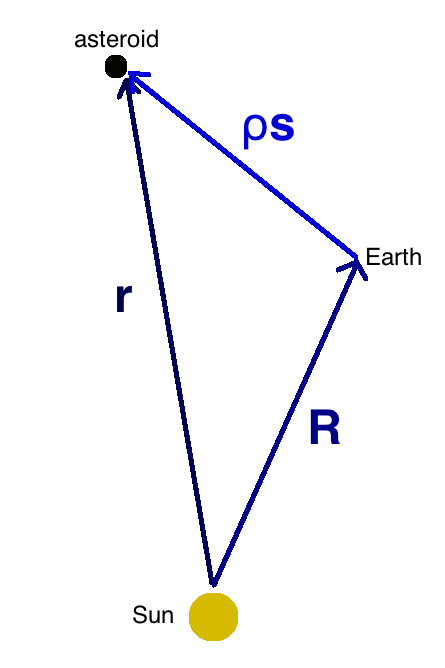
\includegraphics[scale = 0.3]{vectors.png}
\caption{The vector setup used to solve for the asteroid's position relative to the sun.}
\label{fig:vectors}
\end{wrapfigure}

The errors in Table~\ref{tab:pixresid} are already much larger than the residuals between the JPL ephemeris coordinates and those measured from the Dunlap Telescope observations listed in Table~\ref{tab:coords}. These smaller values were processed through all of the transformations needed evaluate orbital elements to demonstrate how even a small deviation from the correct values produces huge discrepancies in the final results.

Proceeding to evaluate the magnitudes of the vector setup as shown in Figure~\ref{fig:vectors} required that all positions be known in the ecliptic plane. Equatorial Cartesian coordinates for Urania were determined from the right ascension and declination values using the same spherical coordinates transformation that had been applied to the Ceres corordinates. Since the equatorial plane of the earth intersects the ecliptic plane at 23.44$^o$, the resulting equatorial coordinates were multiplied by a rotation matrix that corresponded to such a rotation about the mutual x-axis where the two planes intersect.

The position unit vectors were an excellent start, but to proceed further, information about the speed and acceleration of the asteroid was required. To find this information, the first and third of the unit vectors were expressed as Taylor series expansions about the second unit vector ($\mathbf{s_2}$). These two equations were then rearranged to find expressions for the instantaneous velocity ($\mathbf{\dot{s}_2}$) and acceleration vectors ($\mathbf{\ddot{s}_2}$) at the time the of the second measurement. This information, accompanied by measurements of the Earth's position relative to the sun in ecliptic Cartesian coordinates ($\mathbf{R}$~\citep{urania}), was nearly enough to determine the position of the asteroid relative to the sun. It was this position that would ultimately be required in order to predict the asteroid's motion, because it was the sun that was at one of the focii of that orbit. Of course, finding this position would be a matter of simple vector addition if the magnitude of the Earth-asteroid vector was known.

This magnitude was found by iteratively solving two equations that originate in Newton's law of gravity as expressed for both the asteroid and the Earth orbiting the Sun and the differentiated vector equation for $\mathbf{r}$, the vector between the asteroid and sun. The setup of the three vectors is shown in Figure~\ref{fig:vectors}.

\begin{eqnarray}
\label{eqn:rho}
\rho = k^2\left(\frac{1}{R^3}-\frac{1}{r^3}\right)\frac{\mathbf{\dot{s}}\cdot\mathbf{R}\times\mathbf{s}}{\mathbf{\dot{s}}\cdot\mathbf{\ddot{s}}\times\mathbf{s}}\\
\label{eqn:radius}
r^2 = \rho^2 + R^2 + 2\rho\mathbf{R}\cdot\mathbf{s}\\
\dot{\rho} = \frac{k^2}{2}\left(\frac{1}{R^3}-\frac{1}{r^3}\right)\frac{\mathbf{\ddot{s}}\cdot\mathbf{R}\times\mathbf{s}}{\mathbf{\ddot{s}}\cdot\mathbf{\dot{s}}\times\mathbf{s}}
\label{eqn:rhodot}
\end{eqnarray}

In these equations $k = \sqrt{GM_{total}}$, where $G$ is the gravitational constant and $M_{total} \approx M_{sun}$, since $M_{sun} >> M_{earth} >> M_{asteroid}$. $\rho$ is the magnitude of the Earth-asteroid vector, and $r$ is the magnitude of the Sun-asteroid vector. Iteratively solving for these two values using Equations~\ref{eqn:rho} and~\ref{eqn:radius} provided the final pieces needed to determine the position of the asteroid relative to the Sun in ecliptic Cartesian coordinates.

When using the observed coordinates,



%%%%%%%%%%%%%%%%%%%%%%%%%%%%%%%%%%%%%%%%%%

\section{Calculations and Modelling}
\label{sec:calc}

\begin{wrapfigure}{R}{4in}
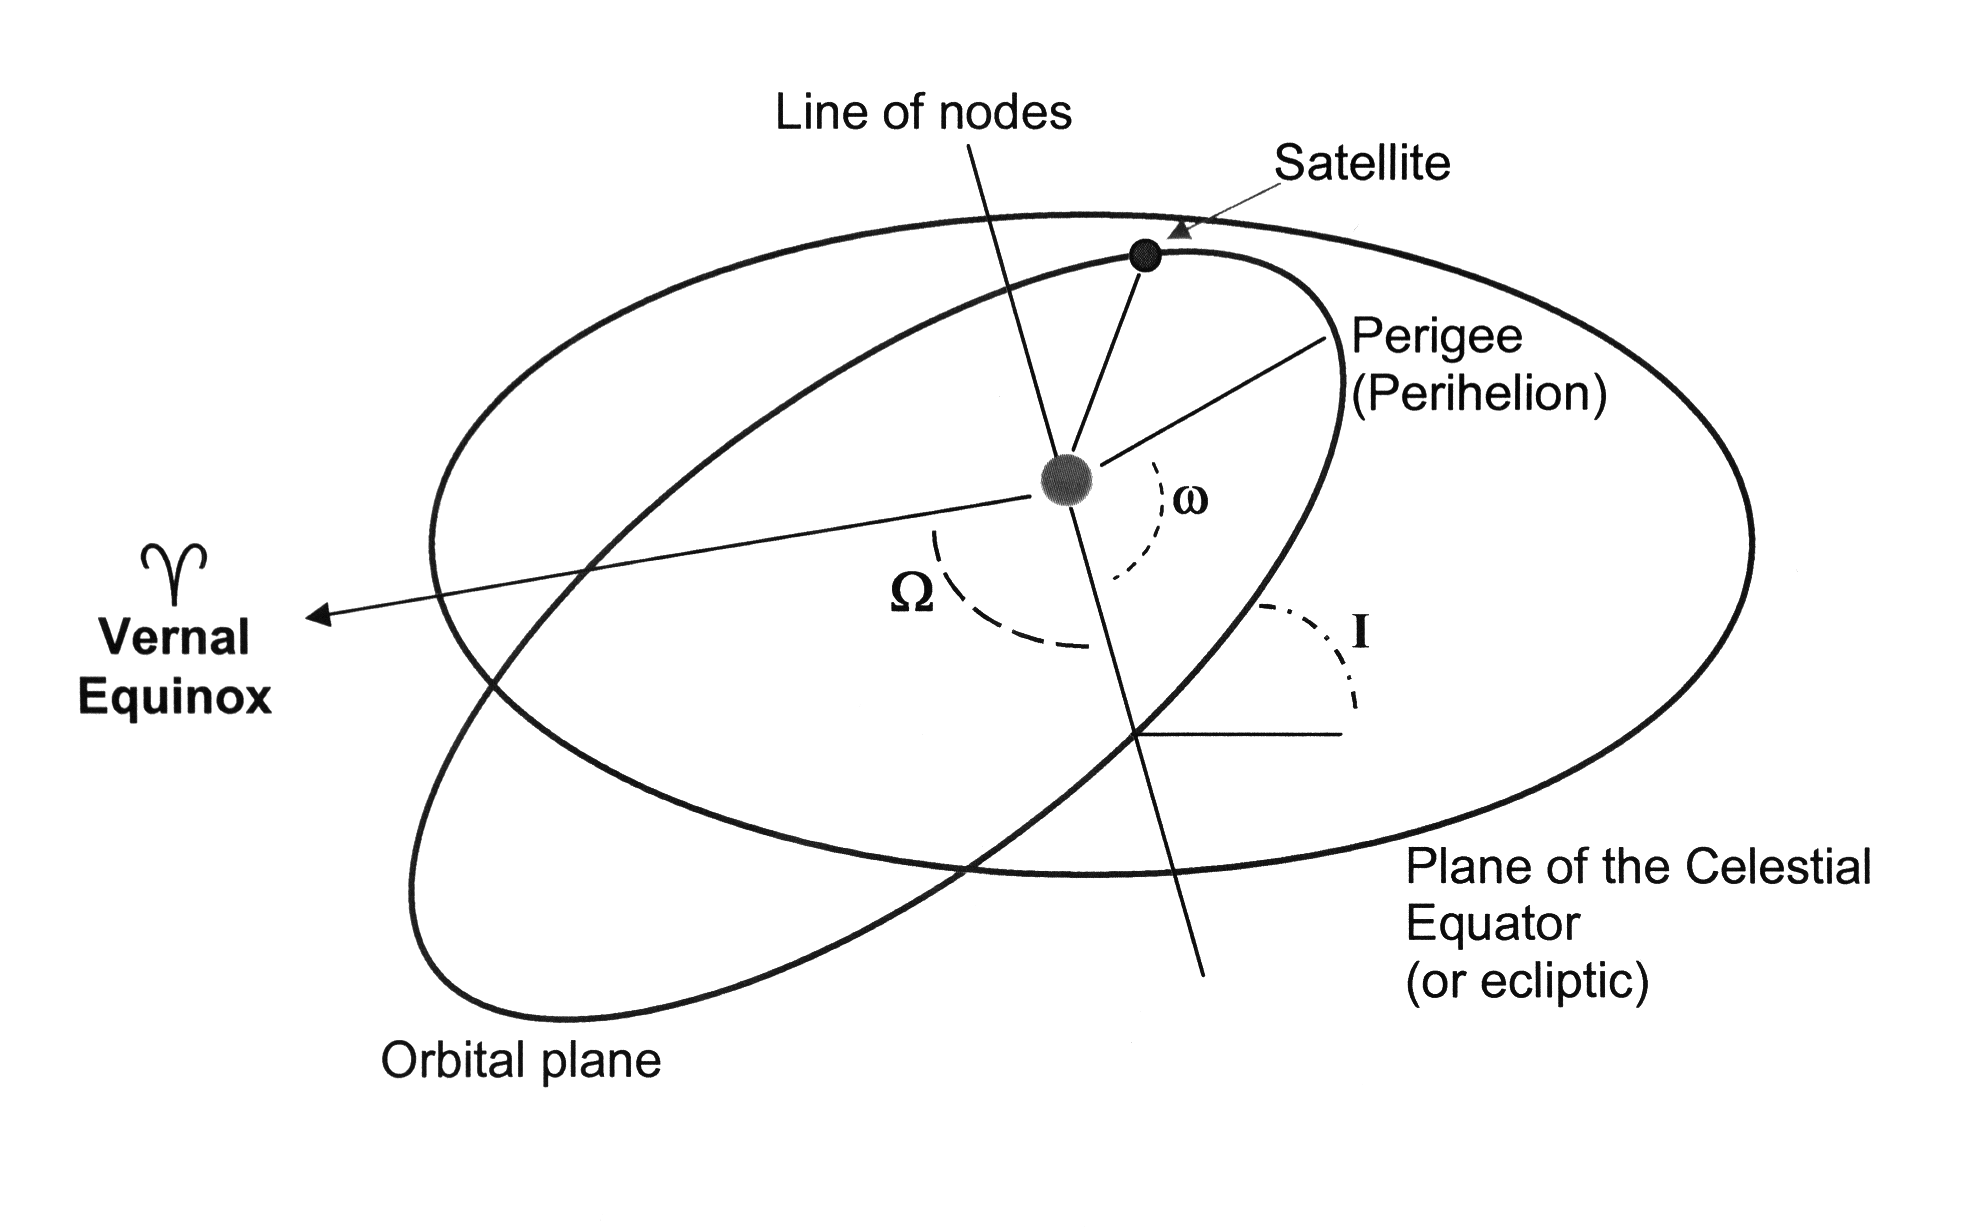
\includegraphics[scale = 0.15]{orbitalelements2.png}
\caption{A diagram illustrating the Keplerian orbital elements \citep{elements}}
\label{fig:elements}
\end{wrapfigure}

After the preliminary work of obtaining the asteroid positions at each epoch, it was possible to define the orbit according to it's Keplerian orbital elements. These elements are, for the most part, illustrated in Figure~\ref{fig:elements}. It was assumed that the orbit of the asteroid was a simple ellipse with the Sun at one of the focci. To characterize the orbit, quite a few parameters were needed. The semi-major axis ($a$, Equation~\ref{eqn:semimajor}), and eccentricity ($e$, Equation~\ref{eqn:eccentricity}), are familiar features of any ellipse. The mean anomaly, eccentric anomaly and true anomaly are all angles that descrive the current position of the asteroid in its orbit



\begin{equation}
a = \frac{k^2r}{2k^2-rV^2}
\label{eqn:semimajor}
\end{equation}

\begin{equation}
tan\Omega = \frac{-h_x}{h_y}
\label{eqn:ascendingnode}
\end{equation}

\begin{equation}
cosi = \frac{h_z}{h}
\label{eqn:inclination}
\end{equation}

\begin{equation}
e = \sqrt{1-(h^2/ak^2)}
\label{eqn:eccentricity}
\end{equation}

\begin{equation}
cosE = \frac{a-r}{ae}
\label{eqn:eccentricanomaly}
\end{equation}

\begin{eqnarray}
\label{eqn:trueanomaly}
tan\left(\frac{\nu}{2}\right) = \sqrt{\frac{1+e}{1-e}}tan\left(\frac{E}{2}\right)\\\
cos(\nu+\omega) = \frac{xcos\Omega + ysin\Omega}{r}
\label{eqn:argperihelion}
\end{eqnarray}

\begin{eqnarray}
\label{eqn:meananomaly}
M = E - esinE\\\
\tau = t - \frac{M}{n}
\label{eqn:timeperihelion}
\end{eqnarray}

\begin{table}[!htbp]
	\centering
	\begin{tabular}{c||c||c||c||c||c||c}
	\hline
	Source & a (AU) & $\Omega$ ($^o$) & i ($^o$) & e & $\omega$ ($^o$) & $\tau$ (Julian Day)\\
	\hline
	True & 2.3650 & 307.93 & 2.0985 & 0.1275 & 86.277 & 2451845\\
	\hline
	JPL & 2.2871 & 308.27 & 2.0841 & 0.1162 & 74.199 & 2455800\\
	\hline
	Observed & 1.2640 & 336.39 & 1.5483 & 0.4511 & 304.87 & 2455754\\
	\end{tabular}
	\caption{}
	\label{tab:elements}
\end{table}

FOV of DI Telescope calculated to be 36.7 arcminutes - not difference so large as to be invisible at the edge. only so good because relatively soon prediction

$\alpha_{JPL}$ = 03:07:15.92, $\delta_{JPL}$ = +19:28:59.7 
$\alpha_{true}$ = 03:06:41.94, $\delta_{true}$ = +19:37:23.1
$\alpha_{obs}$ = 03:08:14.67, $\delta_{obs}$ = +19:43:59.6
%%%%%%%%%%%%%%%%%%%%%%%%%%%%%%%%%%%%%%%%%%

\section{Discussion}
\label{sec:discussion}

\begin{figure}[!htbp]
\centering
\begin{subfigure}{0.5\textwidth}
  \centering
  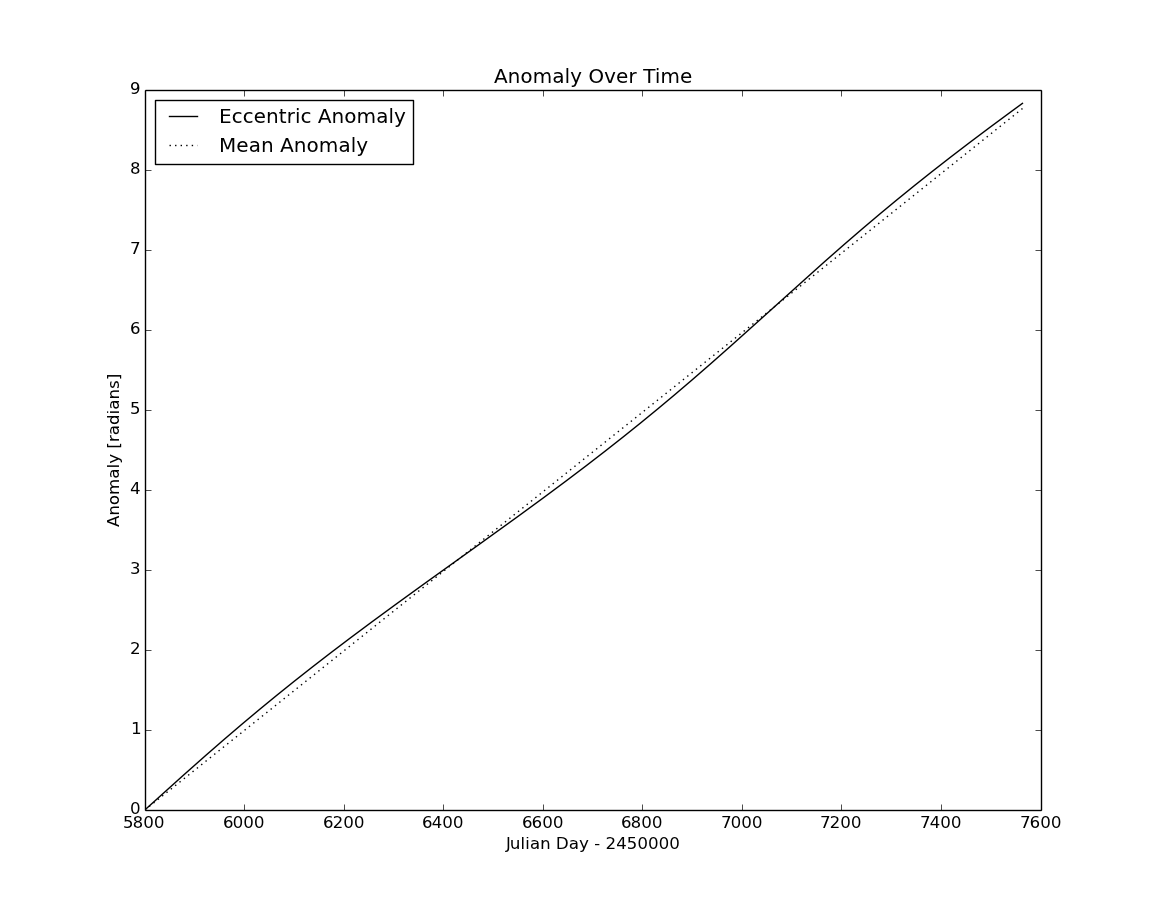
\includegraphics[width=\linewidth]{JPLAnomaly.png}
  \caption{}
  \label{fig:sub1}
\end{subfigure}%
\begin{subfigure}{0.5\textwidth}
  \centering
  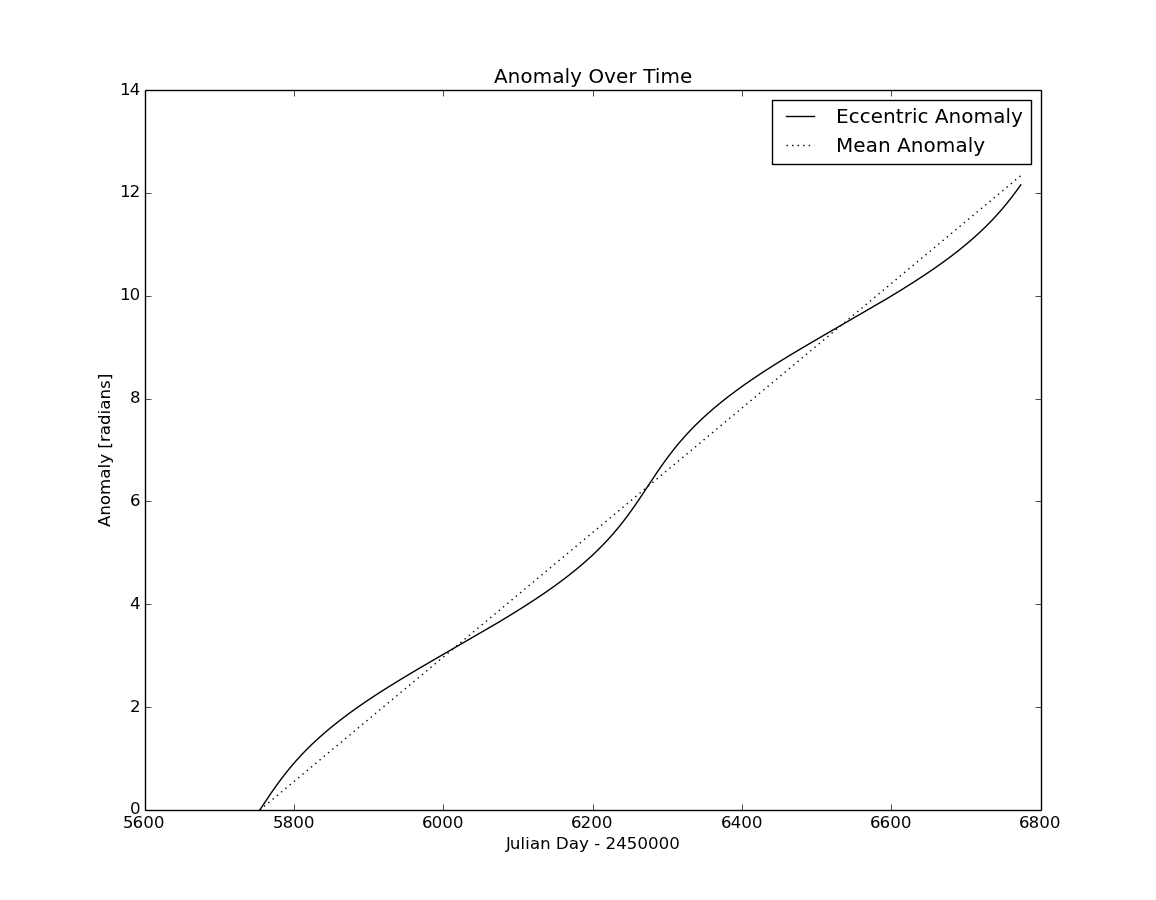
\includegraphics[width=\linewidth]{UraniaAnomaly.png}
  \caption{}
  \label{fig:sub2}
\end{subfigure}
\caption{}
\label{fig:failedFS}
\end{figure}

\begin{figure}[!htbp]
\centering
\begin{subfigure}{0.5\textwidth}
  \centering
  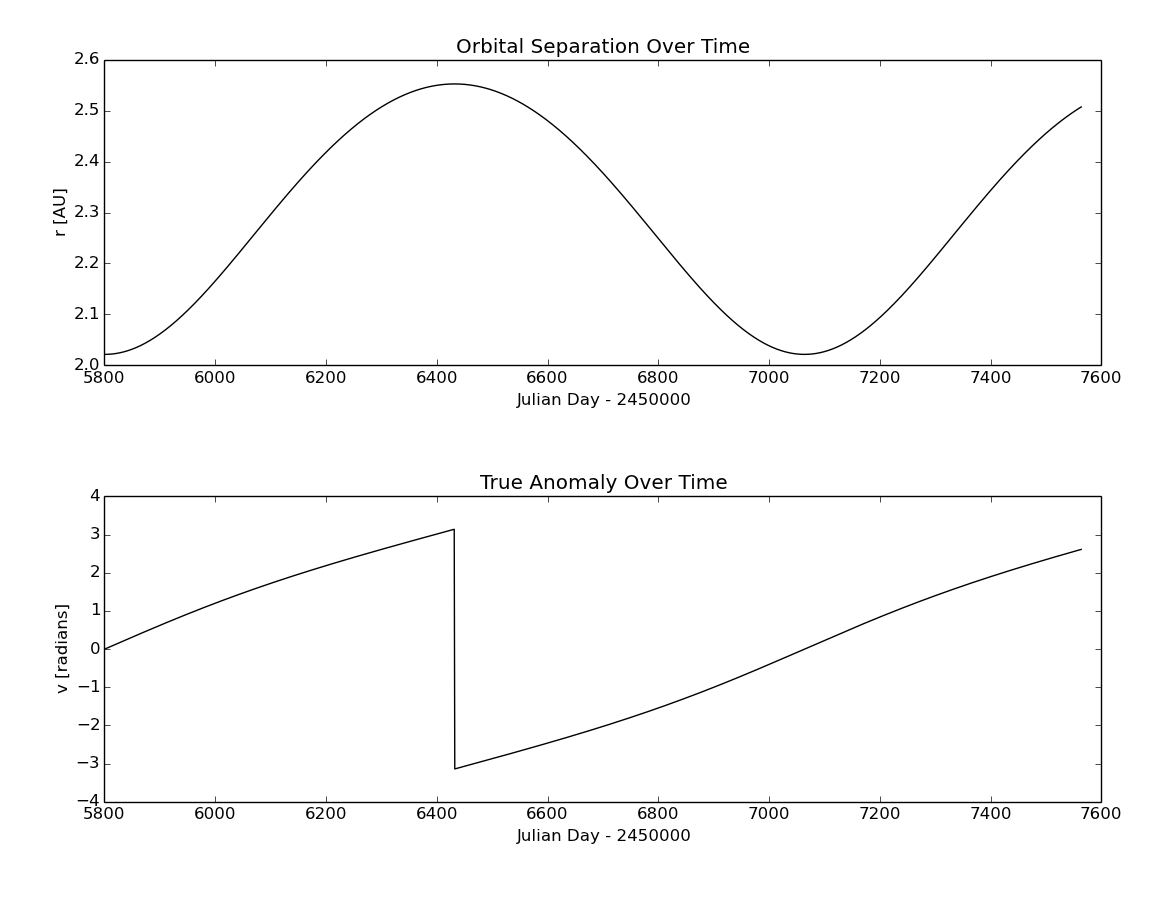
\includegraphics[width=\linewidth]{JPLOrbitalSeparation.png}
  \caption{}
  \label{fig:sub1}
\end{subfigure}%
\begin{subfigure}{0.5\textwidth}
  \centering
  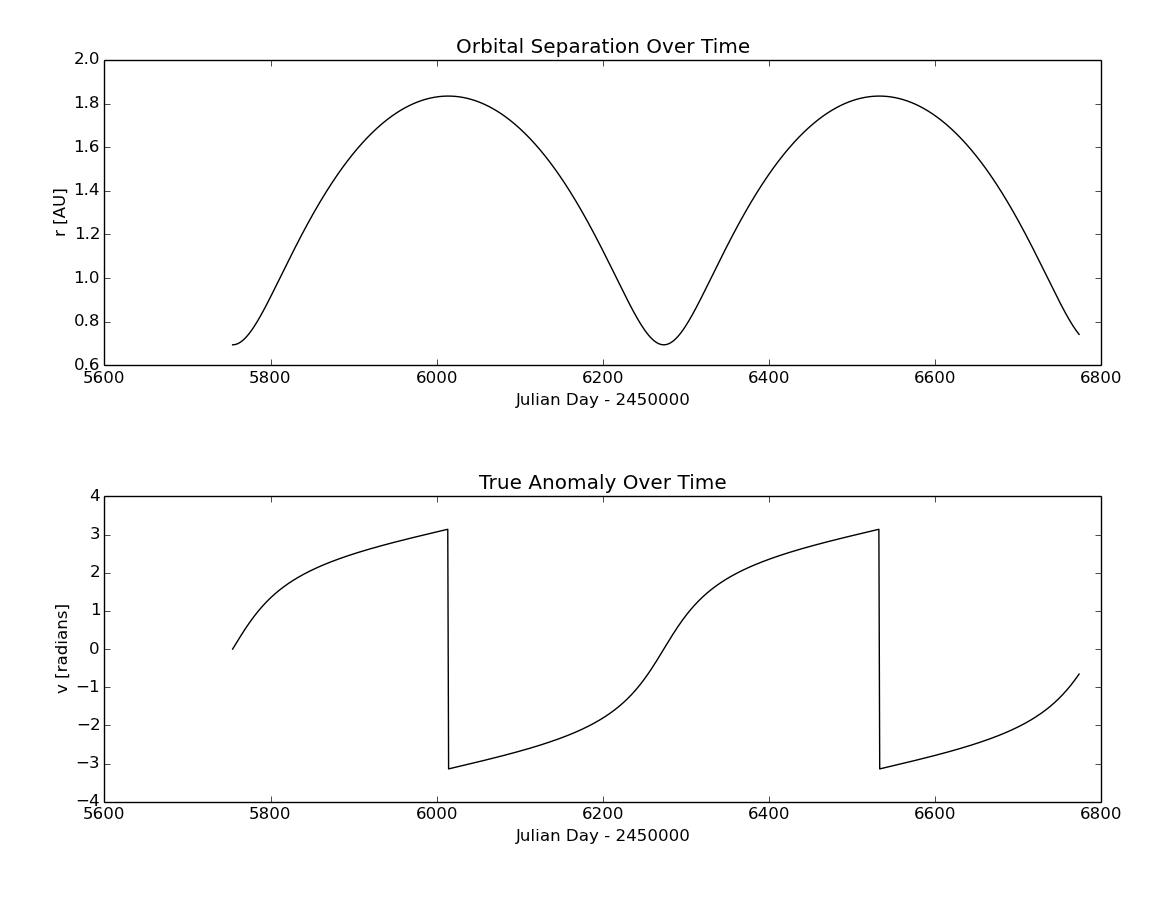
\includegraphics[width=\linewidth]{UraniaOrbitalSeparation.png}
  \caption{}
  \label{fig:sub2}
\end{subfigure}
\caption{}
\label{fig:failedFS}
\end{figure}


\begin{figure}[!htbp]
\centering
\begin{subfigure}{0.5\textwidth}
  \centering
  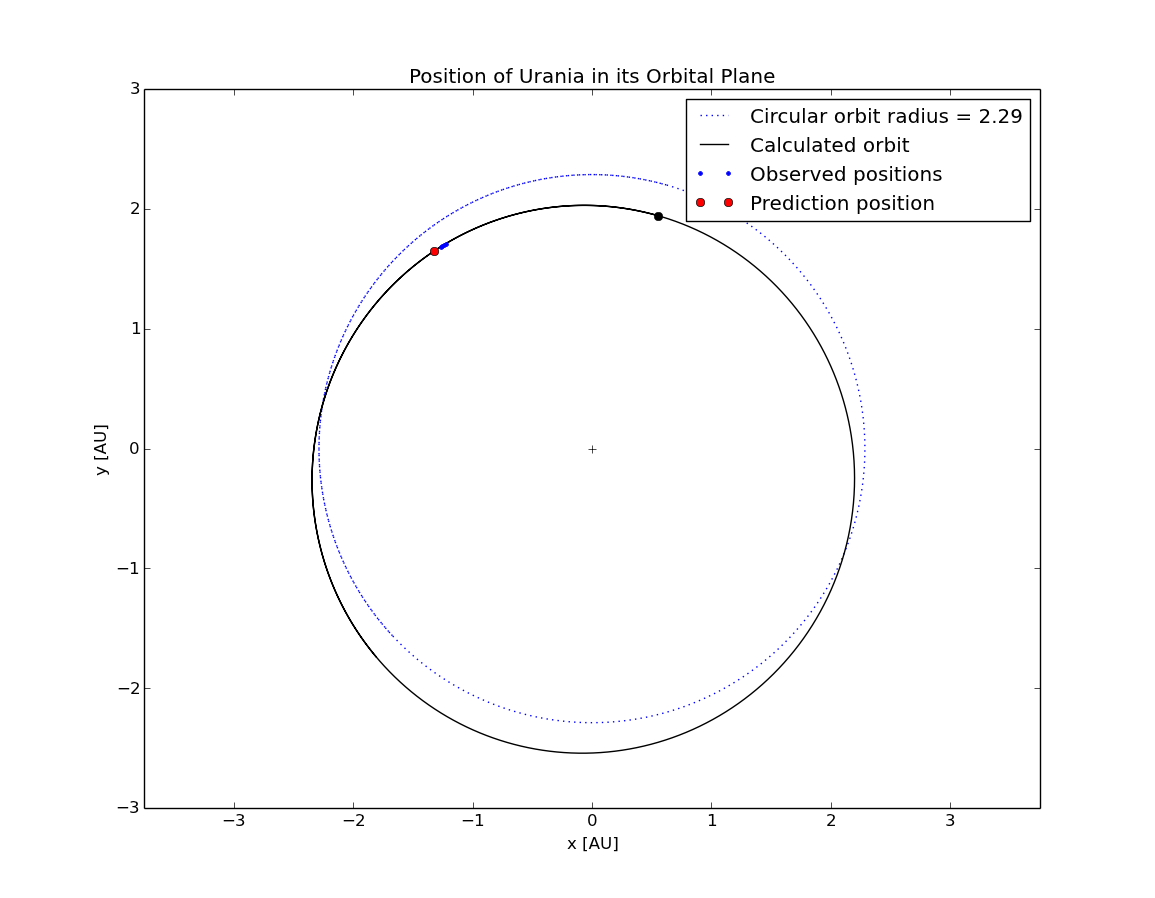
\includegraphics[width=\linewidth]{JPLOrbitalPlane.png}
  \caption{}
  \label{fig:sub1}
\end{subfigure}%
\begin{subfigure}{0.5\textwidth}
  \centering
  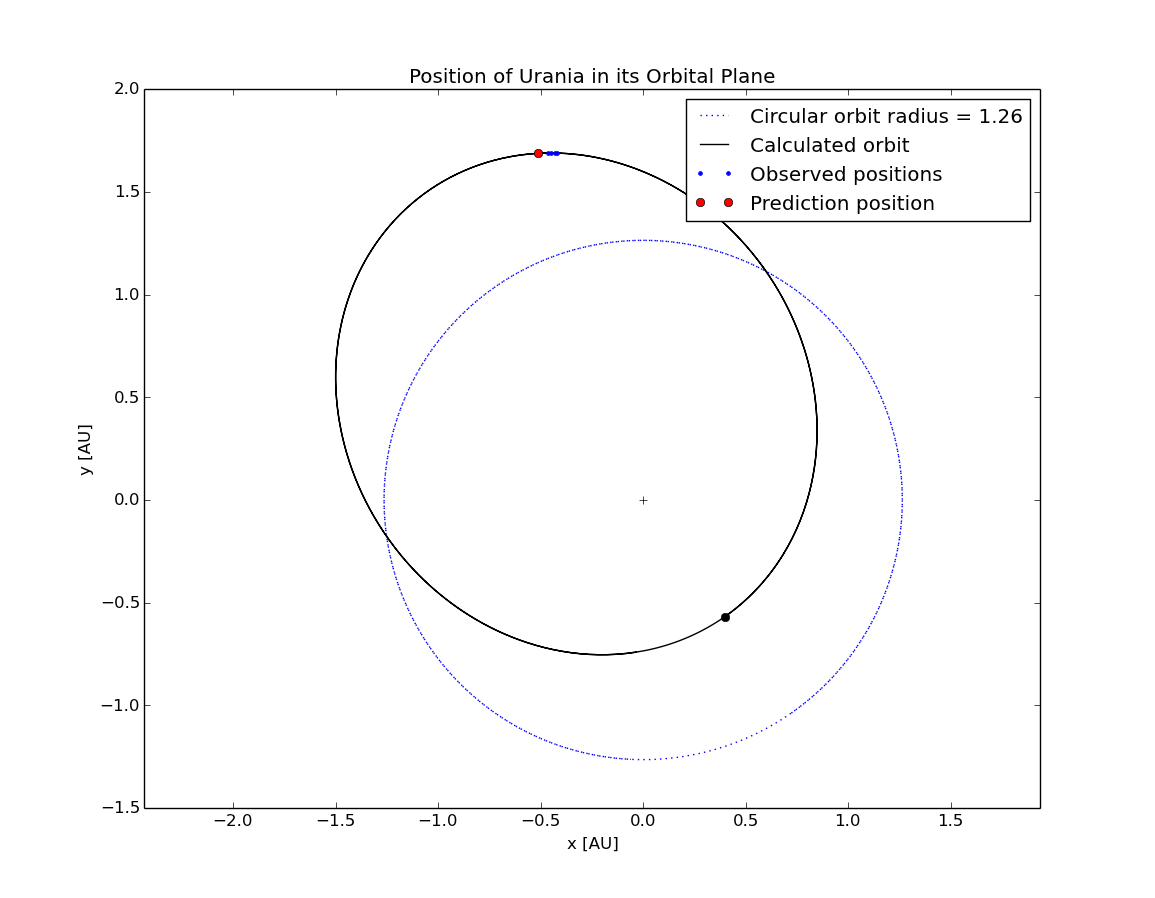
\includegraphics[width=\linewidth]{UraniaOrbitalPlane.png}
  \caption{}
  \label{fig:sub2}
\end{subfigure}
\caption{}
\label{fig:failedFS}
\end{figure}


\bibliographystyle{plainnat}
\bibliography{cite}

\begin{appendices}
%%%%%%%%%%%%%%%%%%%%%%%%%%%%%%%%%%%%%%%%%%%%%%%%%%%%%%%%%%
\section{Plate Constants}
\label{app:plate}

The CCD detector used to observe Urania was not an ideal detector. The pixel coordinates of the asteroid in each image needed to be transformed to more useful right ascension and declination, and this process required the plate constants of the instrument. These values account for possible translation, magnification and rotation of the detector with respect to the sky, and so must be calculated for each observation. This was done by matching centroids found in each night's image with stars from the USNO catalogue. Each centroid was represented by a vector $\vec{x} = (x,y,1)$, and each catalogue star given in standard coordinates by $\vec{X} = (X,Y,1)$. The two were equated with the following matrix multiplier.

\begin{eqnarray}
\mathbf{T} &=& \begin{pmatrix}
(f/p)a_{11}& (f/p)a_{12}& x_{0}\\
(f/p)a_{21}& (f/p)a_{22}& y_{0}\\
0& 0& 1
\end{pmatrix}\nonumber\\
\vec{x} &=& \mathbf{T}\vec{X}\nonumber
\label{eqn:transform}
\end{eqnarray}

The $a_{i}$s in $\mathbf{T}$ are the plate constants. In an ideal case, $\mathbf{T}$ would be the identity matrix, with the final column's two zeroes produced by the central pixel coordinates, $x_{0} = 1024, y_{0} = 1024$. However, solving for the $a_{i}$s produced slightly different results, and it was these plate constants that were used to calculate the position of Urania on each night. The position uncertainty in pixels is listed in Table~\ref{tab:pixresid}

\section{Numerical Solution of Kepler's Equation}

The code below calls multiple functions, which correspond to specific equations listed in the report. The meananomalytime function is Equation~\ref{eqn:timeperihelion} rearranged for M. meananomalyE cooresponds to Equation~\ref{eqn:meananomaly}, and trueanomaly is Equation~\ref{eqn:trueanomaly} solved for $\nu$. ellipseradius is not specified in the body of the text, but is given by $r=a(1-ecosE)$.

\footnotesize\begin{verbatim}
#Calculate the orbital period from Kepler's third law

n = np.sqrt((k**2)/(a**3)) 
period = (2*np.pi)/n

#Generate time intervals

start = tau #time of perihelion
JulianDay = np.arange(start,start+period+500,1)
J = JulianDay - 2450000

#Calculate the initial mean anomaly
M = meananomalytime(n,tau,start)
#Make guess that first eccentric anomaly is equal to the first mean anomaly
E0 = M

#Prepare list to hold stepped out numerical solution for eccentric anomaly
E = []
E.append(E0)

for i in range(1,len(JulianDay)):
  delE = (meananomalytime(n,tau,JulianDay[i]) - meananomalyE(E[i-1],e))/(1-e*np.cos(E[i-1]))
  En = E[i-1] + delE
  E.append(En)

#convert E to a more managable array
E = np.array(E)
#find the mean anomaly at each time
M = meananomalytime(n,tau,JulianDay)

v = trueanomaly(e,E)
r = ellipseradius(E,a,e)

theta = v+omega #omega = argument of perihelion

x_position = r*np.cos(theta)
y_position = r*np.sin(theta)
\end{verbatim}
\normalsize

\end{appendices}

\end{document}